% ================================================================
%  第 3 章 针之所转: Besicovitch 集与 Kakeya 集
%  依据原书 PDF 第 43--62 页译出；编号审计见文件末尾注释
% ================================================================

\chapter{针之所转: Besicovitch 集与 Kakeya 集}

\epigraph{矩形并非有意识的形式. 它是直觉理性的创造. 是新生艺术的面孔. 通往纯粹创造的第一步.}{Kazimir S. Malévich}

\section{认清敌人}

若允许矩形有任意方向，则微分定理竟然是假的——即使对可测集的示性函数亦然——而相应的极大函数对 $L^p$-空间（$1 \leq p < \infty$）中的函数可以几乎处处为无穷. 文献 \cite{b46} 与 \cite{b32} 含有这些事实的证明.

J.~Littlewood 有一个有趣的评论（\cite{b69}，第 392 页）: 他说，为证明一个定理，正确的做法是先找到所要证明之物的最凶恶的敌人，然后引入恰当的假设迫使它改换阵营. Littlewood 为他的原则给出了一个极好的例子: 假设在半带形 $-\pi/2 \leq x \leq \pi/2$，$y \geq 0$ 上有一个解析函数 $F(z)$，在边界上满足 $|F(z)| \leq 1$. 在带形内部是否也有 $|F(z)| \leq 1$?

函数 $F_0(z) = \exp(e^{-iz} - 1)$ 表明答案是否定的. 另一方面，若加上条件: 对某个 $\varepsilon > 0$，$|F(z)| \leq K\exp[\exp((1 - \varepsilon)y)]$，则答案是肯定的，因为这个条件消灭了敌人，并在证明中扮演重要角色. 有趣的是，Littlewood 正是用这一哲学，于 1962 年在他所引的论文中断言: Lulin 关于傅里叶级数几乎处处收敛的猜想应当是错的——而这不过几年之后，Carleson 就给出了著名的证明!

\begin{question}\label{ques:3.1}
求一个面积最小的平面集，在其中可以连续地转动一根针并调换其两端的位置.
\end{question}

这个古怪的问题由日本数学家挂谷宗一（Soichi Kakeya）在一个多世纪前于 \cite{b71} 中提出，如今已成为当代调和分析的核心课题，并且在某种意义上，它与数学分析中最稳固的范式之一——Lebesgue 积分理论——引入了矛盾的因素.

这里的针是 $\R^2$ 中一条长为 $1$ 的有向线段 $\overrightarrow{AB}$. 我们首先想到的能把它转到位置 $\overrightarrow{BA}$ 的集合，是以其中点为心、半径 $1/2$ 的圆，面积为 $\pi/4$. 但这远非问题的解；特别地，还有另一个以星形线为边界的平面集，在其中也可以转动这根针，其面积为 $\pi/8$. 今天我们都知道，这两个集合对回答 Kakeya 的问题都无关紧要，但这一发现属于乌克兰数学家 Abram Besicovitch——几何测度论的创立者之一.

Besicovitch 所关心的是一个稍有不同的问题，为此他构造了 $\R^2$ 中一个闭的有界集，测度为 $0$，在任意方向上都含有一条单位线段. 特别地，该构造蕴含不存在面积最小的这样的集合，因为对每个 $\varepsilon > 0$，都存在面积小于 $\varepsilon$ 的平面集，在其中可以连续地转动一根针并调换两端的位置.

Besicovitch 于动荡的 1919 年在一份不太知名的俄国期刊 \cite{b58} 上发表了论文，当时他并不知道 Kakeya 提出的问题——正如他在多年后发表于 American Mathematical Monthly 的文章 \cite{b62} 中所陈述的那样. 不过，他的动机是不同的，与对 Fubini 定理的理解有关: 该定理对 Lebesgue 积分成立，但对 Riemann 积分方法一般不成立. 不难找到 $\R^2$ 中的函数 $f$，它是 Riemann 可积的（即其不连续点集在 $\R^2$ 中测度为 $0$），但对某个特定值，函数 $x \to f(x, y_0)$ 不是 Riemann 可积的，因为其不连续点集在实直线上有正测度.

一个例子是定义在单位正方形 $Q$ 上的函数 $f$:
\begin{align*}
  f(x,y)=\begin{cases}
  1, & \text{若 } y\neq y_{0},\ \text{其中 } 0<y_{0}<1 \text{ 固定},\\
  1, & \text{若 } y=y_{0} \text{ 且 } x \text{ 为无理数},\\
  0, & \text{若 } y=y_{0} \text{ 且 } x \text{ 为有理数}.
  \end{cases}
\end{align*}
则二重积分 $\iint_{Q} f(x,y) \,\mathrm{d}x\,\mathrm{d}y = 1$ 存在，但 $\int_{0}^{1} \bigl(\int_{0}^{1} f(x,y) \,\mathrm{d}x\bigr) \mathrm{d}y$ 没有意义，因为 $f(x,y_0)$ 不是 Riemann 可积的.

然而，在这个例子中，如果我们足够聪明地旋转坐标轴，困难就消失了.

于是出现下面的问题: 给定 $\R^2$ 中的 Riemann 可积函数，能否选择适当的坐标轴，使二重积分等于累次积分?

Besicovitch 构造的集合给出了否定的回答，而且按照 Littlewood 的说法，它也正是当我们在平面上考虑任意方向矩形上的平均时，Lebesgue 微分定理不成立的主要敌人.

\begin{theorem}\label{thm:3.2}
对每个 $0 < \varepsilon < 1$，存在紧平面集 $K_\varepsilon$，在任意方向上都含有一个 $\varepsilon \times 1$ 的矩形，且其 Lebesgue 测度 $\mu(K_\varepsilon)$ 以 $C/(1 + |\log \varepsilon|)$ 为上界，其中 $C < \infty$ 是普适常数.
\end{theorem}

\begin{proof}
(a) 基本构造. 从一个底边长 $b_0$、高 $h_0$ 的三角形 $T_0$ 出发，用过其底边中点的中线把它分成两个小三角形: $T_0 = T_0^1 \cup T_0^2$.

\begin{center}
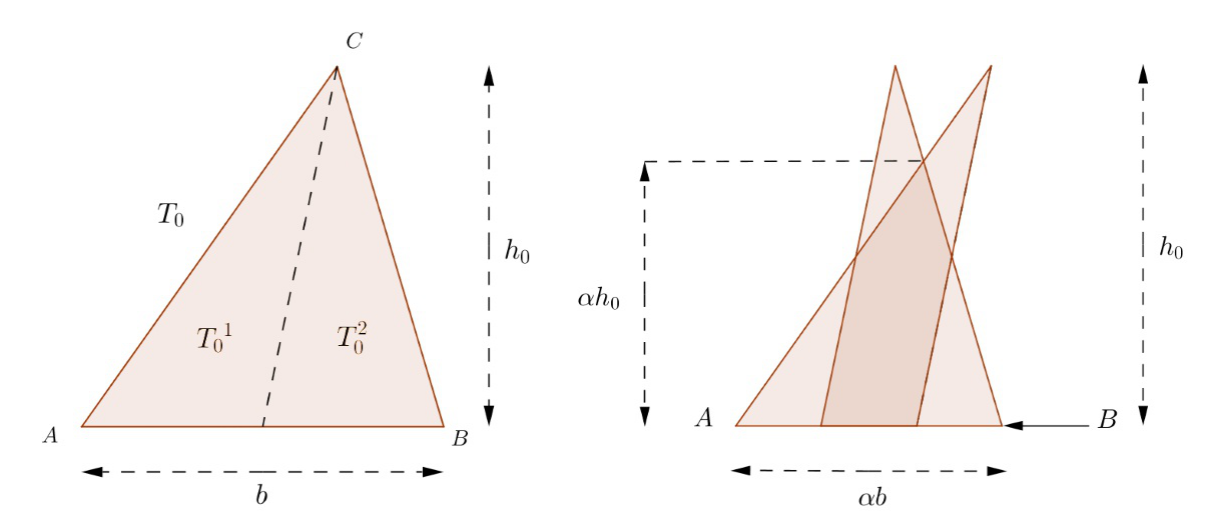
\includegraphics[width=0.6\textwidth]{figs/fig-3-1a.png}
\end{center}

接着，以因子 $\alpha$（$1/2 < \alpha < 1$）平移 $T_0^1$ 与 $T_0^2$，使它们的底边重叠，产生一个图形 $A_1$（树），它由一个与 $T_0$ 相似、比例为 $\alpha$ 的三角形 $T_1$（树干）以及若干树枝 $B_1$ 组成，树枝是与 $T_0^1$ 或 $T_0^2$ 相似、比例为 $1 - \alpha$ 的四个三角形之并.

一个初等计算给出
\begin{align*}
  \mu(A_{1})=\mu(T_{1})+\mu(B_{1})=\bigl(\alpha^{2}+2(1-\alpha)^{2}\bigr)\mu(T_{0})<\mu(T_{0})
\end{align*}
对任何 $1/2 < \alpha < 1$ 成立.

(b) 想法是把基本构造迭代许多次. 现在从高 $h_0$ 的等边三角形 $T_0$ 出发，把其长为 $b_0$ 的底边分成 $2^n$ 个等长 $b_0\,2^{-n}$ 的线段，并把 $T_0$ 分解成 $2^n$ 个小三角形 $T_0^j$，$j = 1, \ldots, 2^n$.

然后对每对 $(T_0^{2k-1}, T_0^{2k})$（$k=1,\ldots,2^{n-1}$），用待定的参数 $\alpha_1$（$1/2<\alpha_1<1$）构造树 $A_1^k=T_1^k\cup B_1^k$，并注意到这些相邻三角形 $T_1^k, T_1^{k+1}$ 中总有两个有两条平行边（不同于它们的底边）. 因此，可以把它们全部平移得到一个新的三角形 $T_1$，与 $T_0$ 相似，底与高分别为 $\alpha_1 b_0$ 与 $\alpha_1 h_0$. 我们还相应地平移各树枝 $B_1^k$，使每个原三角形 $T_0^k$ 在平移后都包含于所得的树 $A_1=T_1\cup\{\text{平移后的树枝}\}$ 中，如上图所示.

\begin{center}
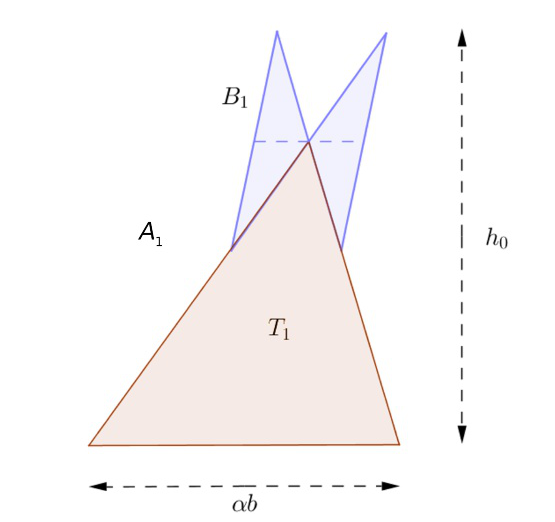
\includegraphics[width=0.36\textwidth]{figs/fig-3-1b.png}
\end{center}

\begin{figure}[htbp]
\centering
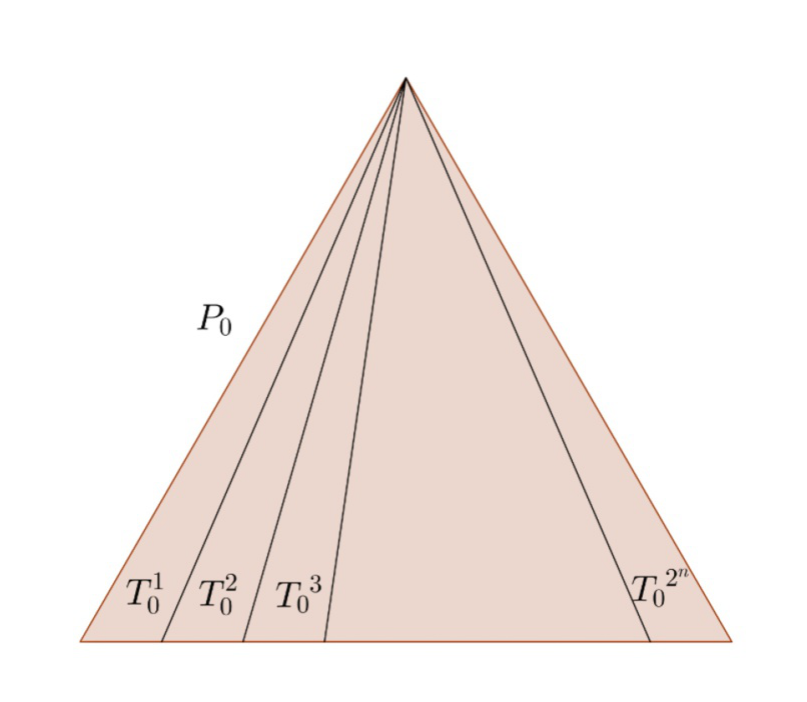
\includegraphics[width=0.5\textwidth]{figs/fig-3-1.png}
\caption{三角形细分.}
\label{fig:3.1}
\end{figure}

我们有
\begin{align*}
  \mu(A_{1})\leq\mu(T_{1})+\mu(B_{1})\leq\{\alpha_{1}^{2}+2(1-\alpha_{1})^{2}\}\mu(T_{0}).
\end{align*}

\begin{figure}[htbp]
\centering
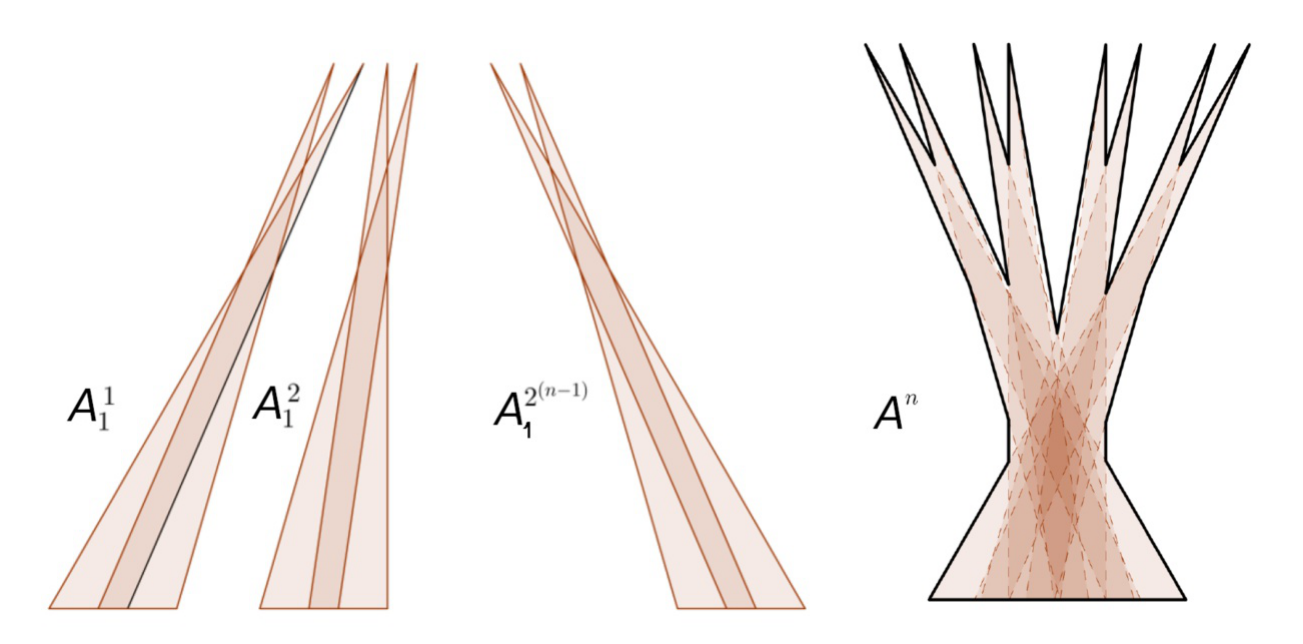
\includegraphics[width=0.66\textwidth]{figs/fig-3-2.png}
\caption{Besicovitch 配对.}
\label{fig:3.2}
\end{figure}

现在注意到 $T_1$ 是 $2^{n-1}$ 个三角形的并，它们的高相等，底长分别为 $\alpha_1 2^{-n+1} b_0$ 与 $\alpha_1 h_0$. 于是可以用另一个比例 $\alpha_2$（$1/2 < \alpha_2 < 1$）重复这一构造，得到第二棵树 $A_2 = T_2 \cup \{\text{树枝}\}$，满足
\begin{align*}
  \mu(A_{2})\leq\left[\alpha_{1}^{2}\alpha_{2}^{2}+2\bigl((1-\alpha_{1})^{2}+\alpha_{1}^{2}(1-\alpha_{2})^{2}\bigr)\right]\mu(T_{0}),
\end{align*}
如此等等.

把这一过程迭代 $n$ 次，产生一棵树 $A_{n}$，使
\begin{align*}
  \mu(A_{n})\leq\{\alpha_{1}^{2}\alpha_{2}^{2}\cdots\alpha_{n}^{2}
  +2[(1-\alpha_{1})^{2}+\cdots+\alpha_{1}^{2}\cdots\alpha_{n-1}^{2}(1-\alpha_{n})^{2}]\}\mu(T_{0}),
\end{align*}
且具有如下性质: 每个原三角形 $T_{0}^{k}$ 都可以平移到 $A_{n}$ 之内.

选取
\begin{align*}
  \alpha_{k}=1-\frac{1}{n+2-k}=\frac{n+1-k}{n+2-k},\qquad k=1,2,\ldots,n,
\end{align*}
给出估计
\begin{align*}
  \mu(A_{n})\leq\frac{2}{n+1}\mu(T_{0}).
\end{align*}
若现在以 $h_0 = 2$ 出发，则集合 $A_n$ 与其按角 $\pi j/3$（$j = 1, 2, 3, 4, 5$）的旋转之并，在适当选取 $n$（即 $2^{-n} \sim \varepsilon$）时给出集合 $K_\varepsilon$.
\end{proof}

显然，在 $K_{\varepsilon}$ 内部，每个平面方向上都放得下一根针. 不过，给 $K_{\varepsilon}$ 添上测度任意小的集合后，我们还能在集合内部连续地移动这根针. 原因是 $K_{\varepsilon}$ 是一些三角形的并，这些三角形的最长边可以成对安排成具有相同的方向，而我们总可以付出任意小的面积，把一条线段在两条平行线之间平移，如下图所示:

\begin{center}
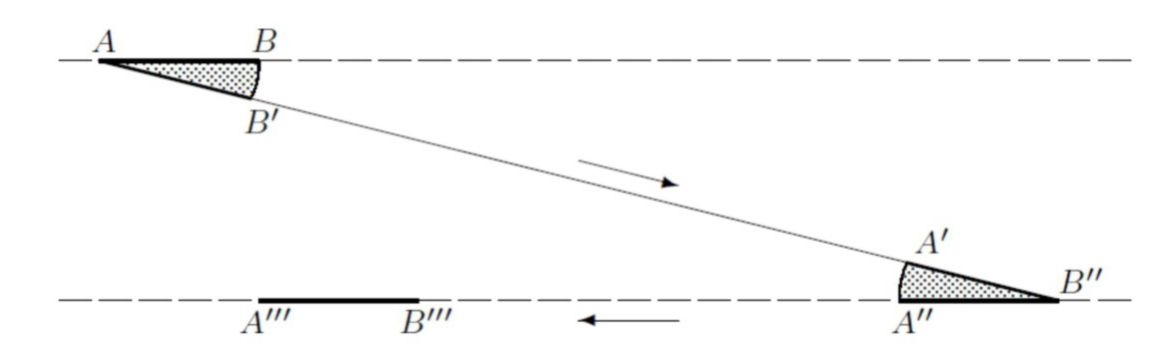
\includegraphics[width=0.55\textwidth]{figs/fig-3-kappa.png}
\end{center}

虚线区域可以做到面积任意小: 只要把平移做得足够远，再利用一条线段在一条直线内移动时产生零面积这一事实即可.

因此，如前所指出的，Kakeya 的原始问题有如下答案: 不存在面积最小的这样的集合，因为对每个 $\varepsilon > 0$，都存在面积小于 $\varepsilon$ 的平面区域，在其中可以转动这根针.

Besicovitch 构造是最优的，如下面的定理所示.

\begin{theorem}\label{thm:3.3}
存在有效常数 $C > 0$，使得若一个平面集在每个方向上都含有一个 $\varepsilon \times 1$ 的矩形（$0 < \varepsilon < 1$），则其面积必大于 $C/[1 + |\log \varepsilon|]$.
\end{theorem}

\begin{proof}
设 $A$ 是这样的集合. 对每个 $j$，$0 \leq j \leq \varepsilon^{-1}$，设 $R_j \subset A$ 是方向（即其最长边的方向）为 $\omega_j = \tfrac{1}{2}\pi\varepsilon j$ 的 $\varepsilon \times 1$ 矩形. Hölder 不等式给出
\begin{align*}
  1\leq\sum_{j}\mu(R_{j})=\int\sum_{j}\chi_{R_{j}}
  \leq\left[\mu\Big(\bigcup_{j}R_{j}\Big)\right]^{1/2}\Big[\sum_{j,k}\mu(R_{j}\cap R_{k})\Big]^{1/2}.
\end{align*}
一个直接的三角计算给出估计
\begin{align*}
  1\leq\left[\mu(A)\right]^{1/2}\Big[\sum_{j,k=1}^{\varepsilon^{-1}}\frac{\varepsilon}{\left|j-k\right|+1}\Big]^{1/2},
\end{align*}
即 $\mu(A) \gtrsim (1 + |\log \varepsilon|)^{-1}$.
\end{proof}

下面我们将修改 Besicovitch 构造，以得到一个极限集 $K$.

\begin{theorem}\label{thm:3.4}
存在测度 $\mu(K) = 0$ 的紧集 $K \subset \R^2$，在每个平面方向上都包含一条单位线段.
\end{theorem}

\begin{proof}
从边长为 $2$ 的等边三角形出发，把其底边分成 $2^{n_0}$ 等份，其中 $n_0$ 取得足够大，使得当我们用参数 $\alpha = 2/3$ 对相邻三角形 $T_0^{2j-1}$，$T_0^{2j}$（$j = 1, \ldots, 2^{n_0-1}$）应用 Besicovitch 的基本构造时，相应的树枝都位于直线 $y = 1$ 上方的区域之内.

我们可以自由地把 $T_0^{2j-1}$ 朝 $T_0^{2j}$ 的方向移动，反之亦然，只有两个极端除外；也就是说，我们希望线段 $AA'BB'$ 包含于所得的三角形 $T_1^1, T_1^2, \ldots, T_1^{2^{n_0}-1}$ 中，从而包含于一族菱形
\begin{align*}
  R_{1}^{\nu_{1}}=T_{1}^{\nu_{1}}\cap\{0\leq y\leq 1\},\qquad \nu_{1}=1,\ldots,2^{n_{0}-1}
\end{align*}
之中. 注意，集合 $\bigcup_{\nu_1} R_1^{\nu_1}$ 在原来三角形的每个方向（即由顶点 $C$ 处的角给出的方向集 $\Gamma$）上都含有一条长度为 $1$ 的直线段，并满足估计
\begin{align*}
  \mu\Big(\bigcup_{\nu_{1}}R_{1}^{\nu_{1}}\Big)\leq\frac{2}{3}\,\mu(R_{0}),
\end{align*}
其中 $R_{0}$ 是以 $AA^{\prime}BB^{\prime}$ 为顶点的菱形.

接着对每个三角形 $T_1^{\nu_1}$ 应用同一过程，得到另一族菱形 $\{R_2^{\nu_1, \nu_2}\}$，使得:
\begin{enumerate}
\item[(i)] $\mu\bigl(\bigcup_{\nu_1, \nu_2} R_2^{\nu_1, \nu_2}\bigr) \leq \bigl(\tfrac{2}{3}\bigr)^2 \mu(R_0)$；
\item[(ii)] 一条长度 $1$、方向属于顶点 $C$ 处原角 $\widehat{ACB}$ 的线段可以放入 $\bigcup_{\nu_1, \nu_2} R_{2}^{\nu_1, \nu_2}$ 之内；
\item[(iii)] $\bigcup_{\nu_1,\nu_2} R_2^{\nu_1,\nu_2}$ 包含所有菱形 $\{R_1^{\nu_1}\}$ 的侧边界线段.
\end{enumerate}
迭代这一过程，对每个 $j = 1,2,\ldots$ 得到一族闭菱形 $\{R_j^{\nu_1,\ldots,\nu_j}\}$ 与一个紧集 $K_j = \bigcup_{\nu_1,\ldots,\nu_j} R_j^{\nu_1,\ldots,\nu_j}$，使得:
\begin{enumerate}
\item[(iv)] $\mu(K_j) \leq \bigl(\tfrac{2}{3}\bigr)^j \mu(R_0)$；
\item[(v)] $K_{j}$ 在原始方向集 $\Gamma$ 的每个方向上都含有一条长度为 $1$ 的线段；
\item[(vi)] 存在稠密的方向集 $\{\theta_e\} \subset \Gamma$，使得对每个 $j = 1, 2, \ldots$，都能在所有的 $K_j$ 中找到一条方向为 $\theta_e$ 的直线段 $I_{\theta_e}$.
\end{enumerate}
令 $K = \bigcap_j K_j$. 则 $K$ 紧，$\mu(K) = 0$，且对每个 $\theta \in \Gamma$，存在一列收敛到 $\theta$ 的上述 $\theta_e$，从而相应的线段 $I_{\theta_e}$ 必收敛到一条方向为 $\theta$ 的线段 $I_\theta$，而由紧性，它也必须包含于集合 $K$ 中.
\end{proof}

\begin{definition}\label{def:3.5}
平面中的\newterm{besicovitch-set}{Besicovitch 集}{Besicovitch set}（或\newterm{kakeya-set}{Kakeya 集}{Kakeya set}）是测度为 $0$、在每个方向上都含有一条定长直线段的集合.
\end{definition}

\begin{corollary}\label{cor:3.6}
平面中 Besicovitch 集的 Minkowski 维数（计盒维数）为 $2$.
\end{corollary}

\begin{proof}
不失一般性，可设 $K$ 在每个方向上都含有长度为 $1$ 的线段. 对每个 $\varepsilon > 0$，集合 $K_{\varepsilon} = \{x : \dist(x, K) \leq \varepsilon\}$ 在每个平面方向上都含有 $\varepsilon \times 1$ 的矩形. 于是
\begin{align*}
  \mu(K_{\varepsilon})\geq\frac{1}{1+|\log\varepsilon|},\qquad
  \lim_{\varepsilon\to 0}\left[2-\frac{\log\mu(K_{\varepsilon})}{\log\varepsilon}\right]=2.
\end{align*}
\end{proof}

\section{Kakeya 极大函数}

设 $N \gg 1$，$\rho > 0$，考虑 $\R^2$ 中所有尺寸为 $\rho \times \rho N$、方向任意的平面矩形组成的族 $\mathcal{B}_N^\rho$. 给定 $\R^2$ 中的局部可积函数 $f$，有极大算子
\begin{align*}
  M_{N}^{\rho}f(x)=\sup_{x\in R\in\mathcal{B}_{N}^{\rho}}\frac{1}{\mu(R)}\int_{R}\left|f(y)\right|\,\mathrm{d}\mu(y).
\end{align*}

\begin{theorem}\label{thm:3.7}
存在有限常数 $C$（与 $N$ 和 $\rho$ 无关），使得对每个 $f \in L^2(\R^2)$ 下列估计成立:
\begin{align*}
  \left\|M_{N}^{\rho}f\right\|_{2}\leq C\left[\log(1+N)\right]^{1/2}\left\|f\right\|_{2}.
\end{align*}
\end{theorem}

\begin{remark}\label{rem:3.8}
只需证明 $\rho = 1$ 的情形，一个方便的膨胀论证即可说明这一点. 由于每个 $R \in \mathcal{B}_N^1$ 都包含于边长为 $N$ 的正方形中，可知 $M_N^1 f(x) \leq N \cdot M f(x)$，其中 $M$ 表示 Hardy--Littlewood 极大函数. 因此，定理的要点不是 $M_N^\rho$ 的有界性，而是其范数的估计 $(\log N)^{1/2}$.
\end{remark}

\begin{proof}[定理~\ref{thm:3.7} 的证明]
族 $\mathcal{B}_N^1$ 可以按其中矩形的方向 $\theta$ 分成两个子族 $\mathcal{B}_{N,1}^1 \cup \mathcal{B}_{N,2}^1$: 对 $\mathcal{B}_{N,1}^1$，$\theta \in [-\pi/4, \pi/4]$；对 $\mathcal{B}_{N,2}^1$，$\theta \in [\pi/4, 3\pi/4]$.

显然，$\mathcal{B}_{N,1}^{1}$ 与 $\mathcal{B}_{N,2}^{1}$ 的相伴极大函数有相同的界. 因此，只须考虑其中之一.

设 $\R^2 = \bigcup_{\nu \in \Z^2} Q_\nu$ 是平面被分成面积 $1$、边平行于坐标轴的不交正方形网格的标准分解.

给定 $f \in L^2(\R^2)$，对每个 $\nu$ 选取矩形 $R_\nu \in \mathcal{B}_{N,1}^1$，满足 $Q_\nu \cap R_\nu \neq \emptyset$ 且
\begin{align*}
  \sup_{x\in Q_{\nu}}M_{N,1}^{1}f(x)\leq 2\,\frac{1}{\mu(R_{\nu})}\int_{R_{\nu}}\left|f(y)\right|\,\mathrm{d}\mu(y),
\end{align*}
即
\begin{align*}
  M_{N,1}^{1}f(x)\leq 2\sum_{\nu}\Big(\frac{1}{N}\int_{R_{\nu}}|f(y)|\,\mathrm{d}\mu(y)\Big)\cdot\chi_{Q_{\nu}}(x).
\end{align*}
于是我们的估计将是下面结果的推论.

\begin{lemma}\label{lem:3.9}
存在有限常数 $C$（与 $N$ 无关），使得对满足 $R_\nu \cap Q_\nu \neq \emptyset$ 的任何矩形 $R_\nu \in \mathcal{B}_{N,1}^1$ 的选取，由公式
\begin{align*}
  T f(x)=\sum_{\nu}\left(\frac{1}{\mu(R_{\nu})}\int_{R_{\nu}}f(y)\,\mathrm{d}y\right)\chi_{Q_{\nu}}(x)
\end{align*}
定义的算子满足估计
\begin{align*}
  \left\|T f\right\|_{2}\leq C\left[1+\log N\right]^{1/2}\left\|f\right\|_{2},\qquad f\in L^{2}(\R^{2}).
\end{align*}
\end{lemma}

\begin{proof}
为证明引理，考虑伴随算子
\begin{align*}
  T^{*}g(x)=\sum_{\nu}\left(\frac{1}{N}\int_{Q_{\nu}}g(y)\,\mathrm{d}y\right)\chi_{R_{\nu}}(x)
\end{align*}
是方便的，并注意到，由于所涉矩形的尺寸是 $1 \times N$，只须检验 $T^*$ 在支于 $N \times N$ 正方形上的函数上的作用.

设 $Q$ 是这样的 $N \times N$ 正方形，边平行于坐标轴. 则 $Q = E_1 \cup \cdots \cup E_N$，其中每个 $E_j$（$j = 1, \ldots, N$）是厚度 $1$ 的竖直带. 对每个 $g \in L^2(Q)$，有 $g = \sum_{j=1}^N g \cdot \chi_{E_j}$，而引理将是估计
\begin{align*}
  \|T^{*}(g\cdot\chi_{E_j})\|_{2}\lesssim N^{-1/2}\left(\log N\right)^{1/2}\|g\cdot\chi_{E_{j}}\|_{2}
\end{align*}
的推论. 为看出这一点，进一步分解 $E_j = \bigcup_{i=1}^{N} Q_i$，其中正方形 $Q_i$ 属于初始网格 $\{Q_\nu\}$，指标 $i$ 表示竖直方向的位置. 再设 $R_i$ 是算子 $T$ 定义中相应指派的 $\mathcal{B}_{N,1}^1$ 矩形. 则
\begin{align*}
  \int|T^{*}(g\cdot\chi_{E_{j}})(x)|^{2}\,\mathrm{d}x
  &\lesssim\sum_{i,k=1}^{N}\frac{1}{N^{2}}\Big(\int_{Q_{i}}|g|^{2}\Big)^{1/2}\Big(\int_{Q_{k}}|g|^{2}\Big)^{1/2}\frac{N}{|i-k|+1}\\
  &\lesssim\frac{1}{N}\left(1+\log N\right)\|g\cdot\chi_{E_{j}}\|_{2}^{2}.
\end{align*}
\end{proof}

\end{proof}

定理 3.7 容许如下的改进: 给定 $N \gg 1$，用 $\mathcal{B}_N$ 表示 $\R^2$ 中离心率（两边长之比）等于 $N$、方向任意的矩形类. 再考虑相伴的极大函数:
\begin{align*}
  M_N f(x)=\sup_{x\in R\in\mathcal{B}_{N}}\frac{1}{\mu(R)}\int_{R}\left|f(y)\right|\,\mathrm{d}\mu(y),
\end{align*}
定义于局部可积函数 $f$ 之上.

\begin{theorem}\label{thm:3.10}
存在有限正常数 $C$ 与 $a$，使得
\begin{align*}
  \left\|M_{N}f\right\|_{2}\leq C(\log N)^{a}\left\|f\right\|_{2}
\end{align*}
对每个函数 $f\in L^{2}(\R^{2})$ 成立.
\end{theorem}

\begin{proof}
首先注意，给定离心率为 $N$ 的任何矩形 $R$，都能找到尺寸相同、方向属于角集 $\{\pi k N^{-1}\}_{k=1,\ldots,N}$ 的另一矩形 $\tilde{R}$，使 $R$ 包含于二倍矩形 $(\tilde{R})^*$ 中. 由此可知，不失一般性，只须对这样的受限方向集 $\{\pi k N^{-1}\}_{k=1,\ldots,N}$ 中的矩形证明上述陈述即可.

用类似的论证，我们还可以假定较短的边长具有形式 $2^n$，$n \in \Z$.

接下来引入如下记号:
\begin{align*}
  T_{2^{n}}^{j}f(x)=\sup_{x\in R}\frac{1}{\mu(R)}\int_{R}\left|f(y)\right|\,\mathrm{d}\mu(y),
\end{align*}
其中上确界取遍所有尺寸为 $2^n \times 2^n N$、方向为 $\pi j N^{-1}$ 的矩形；以及
\begin{align*}
  T_{2^{n}}=\sup_{j}T_{2^{n}}^{j},\qquad
  T^{j}=\sup_{n}T_{2^{n}}^{j},\qquad
  T=\sup_{j}T^{j}=\sup_{n}T_{2^{n}}.
\end{align*}
给定 $\alpha > 0$，可以对每个 $j$ 应用标准（Vitali）覆盖引理，得到一列方向为 $\pi j N^{-1}$、两两不交的矩形 $\{R_l^j\}_{l=1,2,\ldots}$，使得
\begin{align*}
  E_{\alpha}^{j}=\{x:T^{j}f(x)\geq\alpha\}\subset\bigcup_{l}(R_{l}^{j})^{*},\qquad
  \frac{1}{\mu(R_{l}^{j})}\int_{R_{l}^{j}}|f(y)|\,\mathrm{d}\mu(y)\geq\alpha.
\end{align*}
于是，由前述评注，我们知道
\begin{align*}
  E_{\alpha}=\{x:M_{N}f(x)\geq 4\alpha\}\subset\bigcup_{j=1}^{N}E_{\alpha}^{j}.
\end{align*}
设 $n_0$ 是存在尺寸为 $2^{n_0} \times 2^{n_0} N$ 的矩形属于上述序列之一的最大整数，并考虑所有这些矩形组成的族. 我们可以选出具有如下性质的子族 $F_0$: $F_0$ 中没有矩形包含于另一个的二倍矩形之内，而被淘汰的矩形必包含于 $F_0$ 中某个成员的二倍矩形之内.

由归纳，对每个 $k$ 得到一族尺寸为 $2^{n_k} \times 2^{n_k} N$（$n_0 > n_1 > \cdots$）的矩形 $\mathcal{F}_k$，使得 $\mathcal{F}_k$ 中没有矩形包含于 $\mathcal{F}_j$（$j \leq k$）中另一个矩形的二倍矩形之内，且若 $R$ 属于原始的 $N$-族，则 $R$ 要么属于某个 $\mathcal{F}_k$，要么包含于 $\bigcup_k \mathcal{F}_k$ 中某个成员的二倍矩形之内.

由此得
\begin{align*}
  E_{\alpha}\subset\bigcup_{R\in\bigcup_{k}\mathcal{F}_{k}}(R^{*})^{*}.
\end{align*}

接着，对 $k = 0, 1, 2, \ldots$ 定义
\begin{align*}
  \Delta_{k}&=\left\{R\in\bigcup_{j}\mathcal{F}_{j}:\dim(R)=2^{n}\times 2^{n} N;\ n_{0}-k\log N\geq n\geq n_{0}-(k+1)\log N\right\},\\
  E_{i}&=\bigcup_{R\in\Delta_{i}}R,\qquad
  E_{i}^{**}=\bigcup_{R\in\Delta_{i}}\left(R^{*}\right)^{*}.
\end{align*}
注意，集合族 $\{E_i\}$ 是``几乎不交''的，即若 $|i - j| \geq 2$ 则 $E_i \cap E_j = \emptyset$. 这是因为若 $R_1 \in \Delta_i$，$R_2 \in \Delta_j$ 且 $i - j \geq 2$，则 $R_2$ 的最长边小于 $R_1$ 的最短边；又若 $R_1 \cap R_2 \neq \emptyset$，则 $R_2$ 包含于 $R_1^*$，这与我们选取序列 $\mathcal{F}_k$ 的方式矛盾.

令 $f_i = f/E_i$，$i = 0, 1, \ldots$，并设 $S_i$ 是由
\begin{align*}
  S_{i}f(x)=\sup_{x\in R}\frac{1}{\mu(R)}\int_{R}\left|f(y)\right|\,\mathrm{d}y
\end{align*}
定义的极大函数，其中上确界取遍尺寸为 $2^n \times 2^n N$ 的矩形，且
\begin{align*}
  n_{0}+2-i\log N\geq n\geq n_{0}+2-\left(i+1\right)\log N.
\end{align*}
由定理 3.7，我们知道 $S_i$ 在 $L^2(\R^2)$ 上有界，且其范数以 $C(\log N)^{3/2}$ 为界，其中 $C$ 与 $N$ 和 $i$ 无关.

给定 $x \in E_i^{**}$，存在 $R \in \Delta_i$ 使 $x \in (R^*)^*$，从而
\begin{align*}
  S_{i}\,f_{i}(x)\geq\frac{1}{16}\frac{1}{\mu(R)}\int_{R}\left|f_{i}(y)\right|\,\mathrm{d}\mu(y)\geq\frac{\alpha}{16},
\end{align*}
即
\begin{align*}
  E_{i}^{**}\subset\{x:S_{i}f_{i}(x)\geq\alpha/16\},\qquad
  \mu(E_{i}^{**})\lesssim(\log N)^{3}\frac{\|f_{i}\|_{2}^{2}}{\alpha^{2}},
\end{align*}
\begin{align*}
  \mu(E_\alpha)
  &\leq\sum_{i}\mu(E_{i}^{**})
  \lesssim(\log N)^{3}\frac{1}{\alpha^{2}}\int f(x)^{2}\sum_{i}\chi_{E_{i}}(x)\,\mathrm{d}\mu(x)
  \lesssim(\log N)^{3}\frac{1}{\alpha^{2}}\|f\|_{2}^{2},
\end{align*}
即 $M_N$ 满足界为 $\lesssim (\log N)^3$ 的弱 $L^2$ 估计.

由于 $M_N$ 在 $L^\infty$ 上有界且满足界为 $N$ 的弱 $L^1$ 不等式，直接应用 Marcinkiewicz 与 Riesz--Thorin 插值定理即得定理中的强 $L^2$-估计.
\end{proof}

\section{Kakeya 集的 Hausdorff 维数}

给定 Borel 集 $E \subset \R^n$ 以及 $\alpha \geq 0$，$\delta > 0$，定义
\begin{align*}
  H_{\delta}^{\alpha}(E):=\inf\sum[\diam\left(B_{k}\right)]^{\alpha},
\end{align*}
其中下确界取遍 $E$ 的一切由直径小于 $\delta$ 的方体组成的可数覆盖. 再定义
\begin{align*}
  H^{\alpha}(E):=\lim_{\delta\rightarrow 0}H^{\alpha}_{\delta}(E).
\end{align*}
这个极限总是存在，尽管可能为无穷，且具有若干基本性质:
\begin{enumerate}
\item[(1)] $H^\alpha$ 是可数可加的，在平移与旋转下不变，且对 $\lambda > 0$ 满足 $H^\alpha(\lambda E) = \lambda^\alpha H^\alpha(E)$；
\item[(2)] $H^0(E)$ 计数 $E$ 中的点数，而对一切 Borel 集 $E \subset \R^n$，$H^n(E) = c_n \mu(E)$，其中
\begin{align*}
  c_{n}=\frac{\pi^{n/2}}{2^{n}\left(n/2\right)!};
\end{align*}
\item[(3)] 若 $H^{\alpha}(E) < \infty$ 且 $\beta > \alpha$，则 $H^{\beta}(E) = 0$. 若 $\beta < \alpha$ 且 $H^{\alpha}(E) > 0$，则 $H^{\beta}(E) = \infty$.
\end{enumerate}
因此，给定 Borel 集 $E \subset \R^n$，存在唯一的 $\alpha$，使 $\beta > \alpha$ 时 $H^\beta(E) = 0$，$\beta < \alpha$ 时 $H^\beta(E) = \infty$.

\begin{definition}\label{def:3.11}
这个唯一的 $\alpha$ 称为 $E$ 的\newterm{hausdorff-dimension}{Hausdorff 维数}{Hausdorff dimension}. 即
\begin{align*}
  \dim_{H}(E)=\sup\{\beta:H^{\beta}(E)=\infty\}=\inf\{\alpha:H^{\alpha}(E)=0\}.
\end{align*}
\end{definition}

若 Borel 集 $E \subset \R^n$ 有正 Lebesgue 测度，则 $\dim_H(E) = n$.

一个有趣的观察是: 在上述定义中，可以用球或二进方体代替方体，而不改变 $\dim_{H}(E)$ 的值. 而 Minkowski 维数（计盒维数）一般大于 Hausdorff 维数.

\begin{theorem}\label{thm:3.12}
$\R^2$ 中每个 Besicovitch（或 Kakeya）集 $K$ 都满足 $\dim_H(K) = 2$.
\end{theorem}

\begin{proof}
设 $\{Q_\nu\}$ 是由边长 $\ell(Q_\nu) \leq 2^{-k_0}$ 的二进方体组成的 $K$ 的覆盖:
\begin{align*}
  K\subset\bigcup_{\nu}Q_{\nu}=\bigcup_{k=k_{0}}^{\infty}\Big(\bigcup_{\nu}Q_{\nu}^{k}\Big),\qquad
  \text{其中 } \ell(Q_{\nu}^{k})=2^{-k}.
\end{align*}
引入如下记号:
\begin{align*}
  E^{k}=\bigcup_{\nu}Q_{\nu}^{k},\qquad
  N_{k}=\operatorname{Card}\{Q_{\nu}^{k}\}=\text{覆盖中边长为 } 2^{-k} \text{ 的方体数}.
\end{align*}
于是由定义，需要证明
\begin{align*}
  \sum_{k\geq k_{0}}N_{k}2^{-k\alpha}\geq c_{\alpha}>0,\qquad \alpha<2.
\end{align*}
事实上，尝试更强的结论是方便的，即:

\begin{claim*}
对每个 $\alpha < 2$，存在 $k \geq k_0$，使 $N_k 2^{-k\alpha} \geq c_\alpha > 0$.
\end{claim*}

由于 $K$ 是 Besicovitch 集，它对每个方向 $\theta \in S^1$ 都含有长度为 $1$ 的线段 $L_\theta$. 因此
\begin{align*}
  1=\ell(L_{\theta})\leq\sum_{k\geq k_{0}}\ell(L_{\theta}\cap E^{k}).
\end{align*}
于是对每个 $\beta > 0$，存在 $C_{\beta} > 0$ 与 $k \geq k_{0}$，使
\begin{align*}
  \ell(L_{\theta}\cap E^{k})\geq C_{\beta}2^{-k\beta}.
\end{align*}
（这之所以成立，是因为否则将存在 $\beta > 0$，使得对一切 $C_\beta > 0$,
\begin{align*}
  1\leq\sum_{k\geq k_{0}}\ell(L_{\theta}\cap E^{k})\leq C_{\beta}\frac{2^{-k_{0}\beta}}{1-2^{-\beta}},
\end{align*}
而这对足够小的 $C_{\beta}$ 显然不成立.）

给定 $\beta > 0$ 及其相应的 $C_{\beta} > 0$，考虑集合
\begin{align*}
  \Gamma_{k}=\{\theta\in S^{1}:\ell(L_{\theta}\cap E^{k})\geq C_{\beta}2^{-k\beta}\}.
\end{align*}
由此得
\begin{align*}
  1\leq\mu(S^{1})\leq\sum_{k\geq k_{0}}\mu(\Gamma_{k}),
\end{align*}
因为每个角 $\theta \in S^1$ 至少有一个 $k \geq k_0$ 满足
\begin{align*}
  \ell(L_{\theta}\cap E^{k})\geq C_{\beta}2^{-k\beta}.
\end{align*}
于是存在 $k \geq k_0$，使 $\mu(\Gamma_k) \geq C_\beta 2^{-k\beta}$（理由与前面相同: 否则将有不等式
\begin{align*}
  1\leq c_{\beta}\sum_{k\geq k_{0}}2^{-k\beta}=C_{\beta}\frac{2^{-k_{0}\beta}}{1-2^{-\beta}},
\end{align*}
它对足够小的 $C_{\beta}$ 不成立）.

因此，可以在 $\Gamma_k$ 内选取至少 $\frac{1}{2}\,C_\beta\,2^{k(1-\beta)}$ 个不同的角 $\{\theta_j\}$，使得 $j \neq i$ 时 $|\theta_j - \theta_i| \geq 2^{-k}$.

然后考虑这些选定方向的相应线段 $L_{\theta_j}$，并给每条线段配一个方向为 $\theta_j$、尺寸为 $2^{-k} \times 1$ 的矩形 $R_j$. 有下列不等式:
\begin{align*}
  \sum_{j}\mu(R_{j})\geq 2^{-k}\cdot\frac{1}{2}\,C_{\beta}2^{k(1-\beta)}=\frac{1}{2}\,C_{\beta}2^{-k\beta},
\end{align*}
以及
\begin{align*}
  \sum_{j}\mu(R_{j})
  &=\int_{\bigcup_{j}R_{j}}\sum_{j}\chi_{R_{j}}(x)\,\mathrm{d}x
  \leq\mu\Big(\bigcup_{j}R_{j}\Big)^{1/2}\Big[\sum_{j,i}\mu(R_{i}\cap R_{j})\Big]^{1/2}\\
  &\lesssim\mu\Big(\bigcup_{j}R_{j}\Big)^{1/2}
   \Big[\sum_{j,i}\frac{2^{-k}}{|j-i|+1}\Big]^{1/2}
  \lesssim\mu\Big(\bigcup_{j}R_{j}\Big)^{1/2}
   \Big|\log\Big(\tfrac{1}{2}C_\beta 2^{k(1-\beta)}\Big)\Big|^{1/2}.
\end{align*}
即
\begin{equation}\label{eq:3.1}
  \mu\Big(\bigcup_{j}R_{j}\Big)
  \gtrsim\frac{\bigl[\frac{1}{2}C_{\beta}2^{-k\beta}\bigr]^{2}}{\bigl|\log\bigl(\frac{1}{2}C_{\beta}2^{k(1-\beta)}\bigr)\bigr|}
  \geq\widetilde{C}_{\beta}\frac{2^{-2k\beta}}{k},
\end{equation}
其中 $\widetilde{C}_{\beta}>0$.

用 $\mathcal{M}_k$ 表示关于尺寸为 $2^{-k} \times 1$、方向任意的矩形的极大函数，则
\begin{align*}
  \bigcup_{j}R_{j}\subset\{x:\mathcal{M}_{k}(\chi_{E^{k}})(x)\geq C_{\beta}2^{-k\beta}\},
\end{align*}
而由 Kakeya 极大函数所得的估计给出
\begin{align*}
  \mu\Big(\bigcup_{j}R_{j}\Big)\leq\frac{C\left(\log 2^{k}\right)\mu(E^{k})}{C_{\beta}^{2}\,2^{-2k\beta}},
\end{align*}
它与上面得到的估计 \eqref{eq:3.1} 结合，产生不等式
\begin{align*}
  \mu(E^{k})\gtrsim\widetilde{C}_{\beta}\frac{2^{-2k\beta}}{k}\cdot\frac{C_{\beta}^{2}2^{-2k\beta}}{C\left(\log 2^{k}\right)}
  \gtrsim\widetilde{\widetilde{C}}_{\beta}\frac{1}{k^{2}}\,2^{-4k\beta},
\end{align*}
其中 $\widetilde{\widetilde{C}}_{\beta} > 0$ 是某个常数.

另一方面，由于 $E^k$ 是给定覆盖中的二进正方形之并，我们知道 $\mu(E^k) = N_k 2^{-2k}$. 因此,
\begin{align*}
  N_{k}\,2^{-\alpha k}
  \geq 2^{2k}\,\widetilde{C}_{\beta}\,\frac{1}{k^{2}}\,2^{-(4\beta+\alpha)k}
  =\widetilde{C}_{\beta}\,\frac{1}{k^{2}}\,2^{k(2-4\beta-\alpha)}
  \geq C_{\alpha}>0,
\end{align*}
其中 $C_\alpha > 0$ 是某个常数，只要 $2 - 4\beta - \alpha > 0$；对 $\alpha < 2$，这可以对某个 $\beta > 0$ 成立.
\end{proof}

\section{进一步的结果}

\subsection{别的构造}

为构造 Kakeya 集，只须构造测度为零的闭集，使其在一个开角中的每个方向上都含有一条单位线段即可. 因为把它作有限次旋转之并，就满足在每个平面方向上都含有一条直线段的原始要求.

这些集合有另一种构造，归功于 J.-P.~Kahane，见 \cite{b2,b70}.

设 $C$ 是 $x \in [0,1)$ 的 Cantor 集，其中 $x$ 的四进制展开 $x = 0,x_1x_2\ldots x_n\ldots$ 只含数字 $\{0,3\}$. 即把区间 $[0,1)$ 分成四个区间,
\begin{align*}
  [0,1)=[0,1/4)\cup[1/4,1/2)\cup[1/2,3/4)\cup[3/4,1),
\end{align*}
去掉位于中间的两个，对其余两个重复同一程序，如此继续.

令 $C_1 = \frac{1}{2}C = \{\frac{1}{2}x : x \in C\}$，并把 $C$ 与 $C_1$ 的副本分别置于水平直线 $y = 0$ 与 $y = 1$ 上:
\begin{align*}
  C_{1}\subset E_{1}=\{(x,y):0\leq x\leq 1/2,\ y=1\},\qquad
  C\subset E=\{(x,y):0\leq x\leq 1,\ y=0\}.
\end{align*}
定义 $K$ 为把顶部 $C_{1}$ 中的点与底部 $C$ 中的点连接起来的直线段组成的集合. 则有:
$K$ 紧，测度为零，且由连接 $E_{1}$ 中一点与 $E$ 中一点所确定的每个方向上，都含有线段.

\subsection{推广与变体}

定理 3.10 容许若干变体.

设 $\omega_j = (\cos \theta_j, \sin \theta_j)$，$0 \leq \theta_1 < \theta_2 < \cdots < \theta_N \leq \pi$，是``均匀分布''的方向集，意即 $0 < c \leq \theta_{j+1} - \theta_j \leq 2c$，并考虑方向属于 $\{\omega_j\}$ 的矩形族. 则相伴的极大函数 $M$ 满足估计 $\|M f\|_2 \lesssim [1 + \log N]^a \|f\|_2$，其中 $a$ 是与 $N$ 和 $c$ 无关的绝对常数.

文献 \cite{b106} 含有这一结果的证明；把它与 2.5 节缺项情形的结果相比较，可以看出，就极大函数 $L^{2}$-范数的增长而言，均匀分布是最坏的情形. 这一事实由 N.~Katz \cite{b72} 精确化，他证明了对一般的 $N$-平面方向集，对数估计成立.

定理 3.10 还有高维推广: 固定光滑曲线 $\Gamma\colon [0,1] \to S^{n-1}$ 与 $\delta > 0$，考虑方向在曲线 $\Gamma$ 上的 $\delta$-扁针. 则在对 $\Gamma$ 的温和条件下，极大函数的对数估计成立，常数依赖于 $\Gamma$ 但独立于 $\delta > 0$. \cite{b109} 中给出的证明基于归纳论证，并用到了傅里叶变换.

\subsection{高维的部分结果}

Besicovitch 的构造可以在每个维数进行，以产生测度为零、在 $\R^n$ 每个方向上都含有一条单位线段的紧集. 但 Kakeya 极大函数猜想——事实上是本领域的主要问题——在很大程度上仍是公开的，关于这些 Kakeya 集 Hausdorff 维数的估计亦然.

给定 $\delta$，$0 < \delta < 1$，把 $S^{n-1}$ 中的 $\delta$-方向网格定义为集合 $\mathcal{L}_\delta = \{\omega_\alpha\} \subset S^{n-1}$，使得 $\dist(\omega_\alpha, \omega_\beta) \geq \delta$，并且对给定点 $x \in S^{n-1}$，存在 $\omega_\alpha \in \mathcal{L}_\delta$ 满足 $\dist(x, \omega_\alpha) \leq c\delta$，其中 $c \geq 1$ 是固定常数. 显然必须有 $\card(\mathcal{L}_\delta) \simeq \delta^{-(n-1)}$.

有了这样的网格 $\mathcal{L}_{\delta}$，就可以考虑 $\R^{n}$ 中 $\delta$-粗针族 $\mathcal{F}_{\delta}$（高 $1$、半径 $\delta$ 的柱体，或高 $1$、底面边长 $\delta$ 的平行多面体），其方向属于 $\mathcal{L}_{\delta}$.

\begin{conjecture}[$\delta$-粗针猜想]\label{conj:3.13}
设 $\mathcal{A} \subset \mathcal{F}_\delta$ 是 $\mathcal{F}_\delta$ 中方向互不相同的 $\delta$-粗针族. 则下列估计成立:
\begin{align*}
  \int_{\R^{n}}\Big(\sum_{R\in\mathcal{A}}\chi_{R}\Big)^{n/(n-1)}
  \leq C(n)\left[1+|\log\delta|\right]^{a(n)}\sum_{R\in\mathcal{A}}\mu(R),
\end{align*}
其中 $C(n)$ 与 $a(n)$ 与 $\delta$ 无关.
\end{conjecture}

用二维情形的同样论证，我们得到每个 Kakeya 集 Minkowski 维数的精确估计；即
\begin{align*}
  \delta\text{-扁针猜想}\ \Longrightarrow\ \dim K=n.
\end{align*}

\begin{proof}
取 $\delta > 0$，令
\begin{align*}
  K_{\delta}=\{x:\dist(x,K)\leq\delta\}.
\end{align*}
则按定义，$K_\delta$ 在 $\mathcal{L}_\delta$ 的每个方向上都含有一个 $\delta$-粗针. 记这些针的族为 $\mathcal{A}_\delta$. 我们有
\begin{align*}
  1
  &\lesssim\sum_{R\in\mathcal{A}_{\delta}}\mu(R)
  =\int_{K_{\delta}}\sum_{R\in\mathcal{A}_{\delta}}\chi_{R}
  \leq\mu(K_{\delta})^{1/n}\int\Big(\sum_{R\in\mathcal{A}_{\delta}}\chi_{R}\Big)^{n/(n-1)}\\
  &\leq\mu(K_{\delta})^{1/n}\left(C(n)\left[1+|\log\delta|^{a(n)}\right]\right)^{(n-1)/n},
\end{align*}
即 $\dim K = n$.
\end{proof}

在维数 $n \geq 3$ 时，上面的猜想是公开问题. 然而，有一些部分结果给出 Kakeya 集 Minkowski 维数（计盒维数）的下界估计.

\begin{definition}\label{def:3.14}
$\delta$-丛 $\mathcal{B} \subset \mathcal{L}_\delta$ 是方向互不相同、且有公共交点的一族 $\delta$-粗针.
\end{definition}

初等几何的一个简单练习可以证明: 若 $\mathcal{B} = \{R_j\}$ 是 $\delta$-丛，则
\begin{align*}
  \int_{\R^{n}}\Big(\sum_{j}R_{j}(x)\Big)^{n/(n-1)}\mathrm{d}x
  \leq C_{n}\left(1+|\log\delta|\right)\sum_{j}\mu(R_{j}),
\end{align*}
其中 $C_{n}$ 与 $\delta$ 无关.

现在设 $K$ 是 $R^n$ 中的 Kakeya 集，考虑它的 Minkowski 香肠，即
\begin{align*}
  K_{\delta}=\{x\in\R^{n}:\dist(x,K)\leq\delta\},
\end{align*}
它必在网格 $\mathcal{L}_{\delta}$ 的每个方向上都含有一个 $\delta$-针.

设 $\{R_\alpha\}$ 是这些 $\delta$-针组成的族. 给定 $M \geq 1$，可以写
\begin{align*}
  \left\{R_{\alpha}\right\}=B_{0}\cup B_{1}\cup\cdots\cup B_{r},
\end{align*}
其中 $B_0$ 的重叠函数以 $M$ 为界，而每个 $B_j$（$j = 1, \ldots, r$）是基数大于或等于 $M$ 的 $\delta$-丛，于是
\begin{align*}
  r\leq\frac{\delta^{-(n-1)}}{M}.
\end{align*}
然后
\begin{align*}
  \int\Big(\sum_{\alpha}R_{\alpha}\Big)^{n/(n-1)}
  &\lesssim\int\Big(\sum_{R\in B_{0}}R(x)\Big)^{n/(n-1)}
   +r^{1/(n-1)}\sum_{j}\int\Big(\sum_{R\in B_{j}}R(x)\Big)^{n/(n-1)}\\
  &\lesssim\Big[M^{1/(n-1)}+\frac{\delta^{-1}}{M^{1/(n-1)}}\Big]\cdot\mu\Big(\bigcup_{\alpha}R_{\alpha}\Big)|\log\delta|.
\end{align*}
选取 $M^{1/(n-1)} = \delta^{-1/2}$，得到估计
\begin{align*}
  \int\Big(\sum_{\alpha}R_{\alpha}\Big)^{n/(n-1)}\lesssim\delta^{-1/2}\,\mu\Big(\bigcup_{\alpha}R_{\alpha}\Big).
\end{align*}
于是
\begin{align*}
  1
  &\lesssim\sum_{\alpha}\mu(R_{\alpha})
  =\int_{K}\Big(\sum_{\alpha}R_{\alpha}\Big)
  \leq\mu(K_{\delta})^{1/n}\Big(\int\Big(\sum_{\alpha}R_{\alpha}\Big)^{n/(n-1)}\Big)^{(n-1)/n}\\
  &\leq|\log\delta|\;\delta^{-(n-1)/(2n)}\mu(K_{\delta})^{1/n},
\end{align*}
即
\begin{align*}
  \mu(K_{\delta})\gtrsim\frac{\delta^{(n-1)/2}}{|\log\delta|^{n}},
\end{align*}
由此得
\begin{align*}
  \liminf_{\delta\to 0}\left[n-\left|\frac{\log\mu(K_\delta)}{\log\delta}\right|\right]\geq\frac{n+1}{2}.
\end{align*}
即 $K_{\delta}$ 的 Minkowski 维数（计盒维数）大于或等于 $(n+1)/2$.

显然，上面的论证还留有改进的空间，感兴趣的读者可以查阅推荐的文献；在 J.~Bourgain、T.~Wolff、T.~Tao、N.~Katz 与 I.~Laba 等人的文章中，可以找到若干更好的估计. 但它们离猜想值 $n$ 仍很遥远，而后者本可由一个与丛的已知对数估计类似的、针对任何方向互不相同的 $\delta$-粗针族的重叠函数的对数估计推出. 其中一些估计也正是基于对更一般构型——$\delta$-刷——的重叠函数的正确控制.

\begin{definition}\label{def:3.15}
$\delta$-刷 $\mathcal{B} \subset \mathcal{F}_\delta$ 是一族 $\delta$-粗针 $\mathcal{B} = \{R_j\}$，使它们全部与固定的某根（设为 $R_0$）相交，$R_0$ 称为刷的柄.
\end{definition}

\begin{lemma}\label{lem:3.16}
存在有限常数 $C(n)$ 与 $a(n)$，使得 $\R^n$（$n \geq 2$）中的 $\delta$-刷 $\mathcal{B} \subset \mathcal{F}_\delta$ 满足
\begin{align*}
  \int_{\R^{n}}\Big(\sum_{R\in\mathcal{B}}\chi_{R}\Big)^{n/(n-1)}
  \leq C(n)\left[1+|\log\delta|\right]^{a(n)}\sum_{R\in\mathcal{B}}\mu(R).
\end{align*}
\end{lemma}

证明的主要思想是: 刷条件允许把上述不等式化归为熟知的二维情形. 另外，初等几何考虑蕴含:

\begin{lemma}\label{lem:3.17}
给定 $\R^n$ 中的 $\delta$-粗针族 $\mathcal{A}$，满足
\begin{align*}
  \sup_{R\in\mathcal{A}}[\card\{S\in\mathcal{A}:R\cap S\neq\emptyset\}]=M,
\end{align*}
则对每个 $R \in \mathcal{A}$,
\begin{align*}
  \int_{R}\Big(\sum_{S\in\mathcal{A}}\chi_{S}\Big)^{1/(n-1)}
  \leq C(n)\left[1+|\log\delta|\right]^{a(n)}
  M^{(n-2)/(n-1)^{2}}\,\delta^{n-1}.
\end{align*}
\end{lemma}

\begin{proposition}\label{prop:3.18}
上述两个引理的结合给出任何 Kakeya 集 Minkowski 维数 $\geq (n+2)/2$ 的估计.
\end{proposition}

\begin{proof}
考虑 Minkowski 香肠 $K_\delta$，它在球面网格 $\mathcal{L}_\delta$ 的每个方向上都含有一个 $\delta$-粗针. 若 $\{R_\alpha\}$ 是这些 $\delta$-针组成的族，则有分解
\begin{align*}
  \left\{R_{\alpha}\right\}=\mathcal{B}_{1}\cup\mathcal{B}_{2}\cup\cdots\cup\mathcal{B}_{m},
\end{align*}
其中在这个不交并中每个 $B_j$ 都是基数递减的 $\delta$-刷.

给定待定的 $\lambda \geq 1$，考虑 $r(\lambda)$，使对 $j > r(\lambda)$ 有
\begin{align*}
  \card(\mathcal{B}_{j})\leq\lambda\,\delta^{-(n-1)/2},
\end{align*}
这就给出
\begin{align*}
  r(\lambda)\leq\frac{1}{\lambda}\,\delta^{-(n-1)/2}.
\end{align*}
于是有分解
\begin{align*}
  \{R_{\alpha}\}=\mathcal{B}^{*}\cup\mathcal{B}^{**},\qquad
  \mathcal{B}^{*}=\bigcup_{j=1}^{r(\lambda)}\mathcal{B}_{j}.
\end{align*}
Hölder 不等式与引理 3.16 给出
\begin{align*}
  \int\Big|\sum_{R\in\mathcal{B}^{*}}\chi_{R}\Big|^{n/(n-1)}
  \leq C(n)\left(1+|\log\delta|\right)^{a(n)}
  \frac{\delta^{-1/2}}{\lambda^{1/(n-1)}}\sum_{R\in\mathcal{B}^{*}}\mu(R).
\end{align*}
另一方面，引理 3.17 给出
\begin{align*}
  \int\Big|\sum_{R\in\mathcal{B}^{**}}\chi_{R}\Big|^{n/(n-1)}
  &=\sum_{R\in\mathcal{B}^{**}}\int_{R}\Big|\sum_{R\in\mathcal{B}^{**}}\chi_{R}\Big|^{1/(n-1)}\\
  &\leq C(n)[1+|\log\delta|]^{a(n)}
   \lambda^{\frac{n-2}{(n-1)^{2}}}\,\delta^{-\frac{n-2}{2(n-1)}}\sum_{R\in\mathcal{B}^{**}}\mu(R).
\end{align*}
现在选取 $\lambda = \delta^{-1/2}$，得到估计
\begin{align*}
  \int\Big|\sum_{\alpha}\chi_{R_{\alpha}}\Big|^{n/(n-1)}
  \leq C(n)[1+|\log\delta|]^{a(n)}
  \delta^{-\frac{n-2}{2(n-1)}}\sum_{\alpha}\mu(R_{\alpha}),
\end{align*}
以及
\begin{align*}
  1\lesssim\sum_{\alpha}\mu(R_{\alpha})
  \lesssim\mu(K_{\delta})^{1/n}\left[C(n)\left(1+|\log\delta|\right)^{a(n)}\right]^{(n-1)/n}
  \delta^{\frac{n-2}{2n}},
\end{align*}
由此得到
\begin{align*}
  n-\limsup_{\delta\to 0}\frac{\log\mu(K_{\delta})}{\log\delta}\geq\frac{n+2}{2}.
\end{align*}
\end{proof}

\begin{proof}[引理~\ref{lem:3.16} 的证明]
第一个发表的证明见 \cite{b77}. 下面是出自我七十年代笔记的概要版.

首先，为简化几何，不失一般性可假定: 对柄为 $R_0$ 的刷中的每个 $R_j$，$R_j \setminus (R_0 \cap R_j)$ 是连通的，且刷中每根针 $R_j$ 的轴都与 $R_0$ 的轴相交.

用 $M(\delta)$ 表示不等式
\begin{align*}
  \int\Big|\sum_{R\in\mathcal{B}}\chi_{R}\Big|^{n/(n-1)}
  \leq M(\delta)\sum_{R\in\mathcal{B}}\mu(R)
\end{align*}
对所有这样的 $\delta$-刷成立的最佳常数，并注意由膨胀，若考虑高为 $h$、半径 $\delta h$（$h > 0$ 固定）的柱体，常数相同.

设 $\mathcal{B} = \{R_0, R_1, \ldots, R_\gamma\}$ 是 $\delta$-刷（这里高取为 $1$），柄为 $R_0$，即 $R_j \cap R_0 \neq \emptyset$ 且 $R_j \setminus (R_0 \cap R_j)$ 连通. 考虑到形如 $|\log \delta|$ 的因子对维数估计无关紧要，不失一般性可设 $\gamma$ 含于区间 $2^{-m(n-1)} \leq \gamma < 2^{-(m-1)(n-1)}$，使得
\begin{align*}
  2^{(m-1)}\delta\leq\operatorname{angle}(R_{j},R_{0})<2^{m}\delta.
\end{align*}

接着把刷中的每个 $R_j$ 分成两半 $R_j^1 \cup R_j^2$，其中 $R_j^1 \cap R_0 \neq \emptyset$. 我们有
\begin{align*}
  \int\Big(\sum_{j}\chi_{R_{j}^{2}}\Big)^{n/(n-1)}
  =\sum_{j}\int_{R_{j}^{2}}\Big(\sum_{k}\chi_{R_{k}^{2}}\Big)^{1/(n-1)},
\end{align*}
并注意对每个 $j$，族 $\{R_k^2 : R_k^2 \cap R_j^2 \neq \emptyset\}$ 分成有限（与 $\delta$ 无关）个部分，使得在每一部分上，$R_k^2 \cap R_j^2 \neq \emptyset$ 蕴含 $R_k$ 的方向有 $n - 2$ 个坐标固定. 因此，可以用 $L^2$-估计证明
\begin{align*}
  \sum_{j}\int_{R_{j}^{2}}\Big(\sum_{k}\chi_{R_{k}^{2}}\Big)^{1/(n-1)}
  \lesssim|\log\delta|^{a(n)}\sum_{j}\mu(R_{j}^{2}).
\end{align*}
关于 $\sum_{k}\chi_{R_k^1}$，注意每个 $R_k^1$ 是 $(2\delta)$-粗针，且 $\sum_{k}\chi_{R_k^1}$ 至多分成 $2^{n-1}$ 个 $(2\delta)$-粗刷 $\mathcal{B}_\alpha^*$. 因此,
\begin{align*}
  \int\Big|\sum_{k}\chi_{R_{k}^{1}}\Big|^{n/(n-1)}
  \lesssim\big[M(2\delta)+|\log\delta|^{a(n)}\big]\sum_{R\in\mathcal{B}}\mu(R),
\end{align*}
而递推公式
\begin{align*}
  M(\delta)\leq M(2\delta)+|\log\delta|^{a(n)}
\end{align*}
给出所要的估计.
\end{proof}

\begin{proof}[引理~\ref{lem:3.17} 的证明]
不失一般性，可以假设 $M = 2^{m(n-1)}$，$m = 0,1,\ldots,-\log_2\delta$. 此外，给定这样的 $M$，显然积分
\begin{align*}
  \int_{R}\Big(\sum_{S\in\mathcal{A}}S\Big)^{1/(n-1)}
\end{align*}
在 $\mathcal{A}$ 中与 $R$ 相交的一切针 $S$ 都满足角 $(R, S) \leq 2^m \delta$ 时达到最大.

接着，把集合 $\{S \in \mathcal{A} : S \cap R \neq \emptyset\}$ 至多分成 $-\log_2 \delta$ 个类 $\mathcal{A}_j(R)$，由 $2^j \delta \leq \operatorname{angle}(S, R) < 2^{j+1} \delta$ 定义，并注意
\begin{align*}
  S\in\mathcal{A}_{j}(R)\ \Longrightarrow\ \mu(R\cap S)\leq\frac{\delta^{n-1}}{2^{j}}.
\end{align*}
把 $R$（沿其高）分成 $2^j$ 段长度为 $2^{-j}$ 的针,
\begin{align*}
  R=\bigcup_{i=1}^{2^{j}}R_{i},
\end{align*}
并记 $c_i = \card\{S \in \mathcal{A}_j(R) : S \cap R_i \neq \emptyset\}$. 则
\begin{align*}
  \int_{R}\Big(\sum_{S\in\mathcal{A}_{j}(R)}\chi_{S}\Big)^{1/(n-1)}
  &\lesssim\Big(\sum_{i=1}^{2^{j}}c_{i}\Big)^{1/(n-1)}\frac{\delta^{n-1}}{2^{j}}\\
  &\lesssim\Big(\sum_{i}c_{i}\Big)^{1/(n-1)}2^{j\frac{n-2}{n-1}}\frac{\delta^{n-1}}{2^{j}}
  \lesssim 2^{j\frac{n-2}{n-1}}\delta^{n-1},
\end{align*}
把这些 $j \leq m$ 的估计相加即得结果.
\end{proof}

这些几何的或至上主义的方法可以再精细，但似乎仍不足以得到该猜想. 1999 年，J.~Bourgain 发明了一种新方法，基于集合之和与差之算术组合学，它给出高维的若干改进，并把 Kakeya 猜想与数论中关于 Dirichlet 级数的其他猜想建立了有趣的联系.

% ================================================================
% 编号审计 (第 3 章):
%   question ques:3.1 → 问题 3.1  (§3.1，Kakeya 问题)
%   theorem  thm:3.2  → 定理 3.2  (§3.1)
%   theorem  thm:3.3  → 定理 3.3  (§3.1)
%   theorem  thm:3.4  → 定理 3.4  (§3.1)
%   definition def:3.5 → 定义 3.5 (§3.1，Besicovitch/Kakeya 集)
%   corollary cor:3.6 → 推论 3.6  (§3.1)
%   theorem  thm:3.7  → 定理 3.7  (§3.2，Kakeya 极大函数)
%   remark   rem:3.8  → 注 3.8    (§3.2)
%   lemma    lem:3.9  → 引理 3.9  (§3.2)
%   theorem  thm:3.10 → 定理 3.10 (§3.2)
%   definition def:3.11 → 定义 3.11 (§3.3，Hausdorff 维数)
%   theorem  thm:3.12 → 定理 3.12 (§3.3)
%   conjecture conj:3.13 → 猜想 3.13 (§3.4.3，δ-粗针猜想)
%   definition def:3.14 → 定义 3.14 (§3.4.3，δ-丛)
%   definition def:3.15 → 定义 3.15 (§3.4.3，δ-刷)
%   lemma    lem:3.16 → 引理 3.16 (§3.4.3)
%   lemma    lem:3.17 → 引理 3.17 (§3.4.3)
%   proposition prop:3.18 → 命题 3.18 (§3.4.3)
%   公式: eq:3.1 (定理 3.12 证明中的下界)
%   无编号 Claim 用 claim* 环境 (定理 3.12 证明内).
%   注: 定理 3.4 证明中的"移动线段"插图(fig-3-2b 引用)与 §3.1 尾部
%       无编号图(fig-3-1a，fig-3-1b，fig-3-kappa)均为无编号图.
%   \cite 使用: b2 b32 b46 b58 b62 b69 b70 b71 b72 b77 b106 b109
% ================================================================
